\section{Auswertung}
\label{sec:Auswertung}

Die im Versuch aufgenommenen Daten dienen nun zur Bestimmung der Aktivierungsenergie $W$ und der charakteristischen Relaxationszeit $\tau_0$.

In \autoref{fig:plot1} ist zunächst der gemessene Relaxationsstrom in Abhängigkeit von der Temperatur aufgetragen.

\begin{figure}[H]
  \centering
  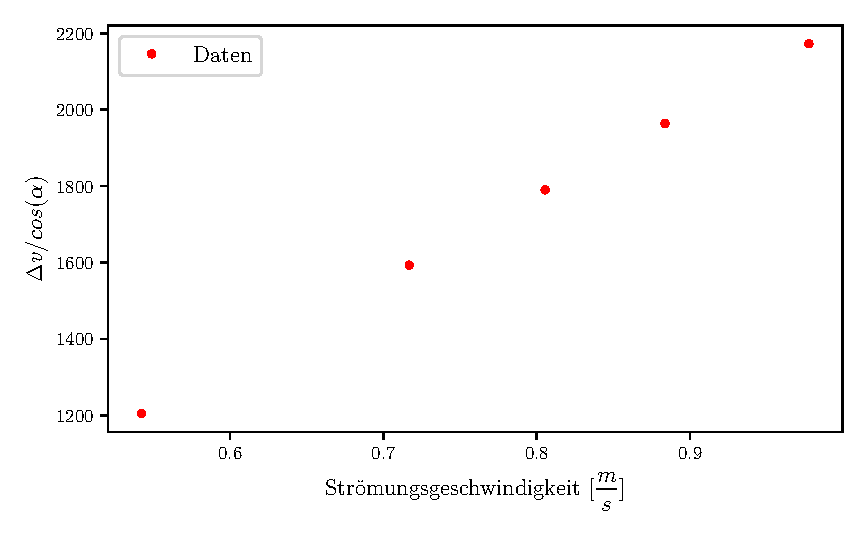
\includegraphics[width=\textwidth]{build/plot1.pdf}
  \caption{Depolarisationsstrom in Abhängigkeit von der Temperatur mit Regression für den Untergrund.}
  \label{fig:plot1}
\end{figure}

Die mittlere Heizrate berechnet sich zu
%\begin{align*}
%  b= \qty{}{\kelvin\per\minute}.
%\end{align*}

Da das erste Maximum des Relaxationsstroms, welches im Folgenden genauer
untersucht wird, auf der steigenden Flanke des zweiten Maximums liegt, wird dieser
”Untergrund” von den Messwerten abgezogen.
Um den Untergrund zu bestimmen wird eine Regression der Form
\begin{align*}
  f(T)= a * \text{exp}(-b/T)
\end{align*}
an den Messwerten durchgeführt die außerhalb der Maximumskurve liegen.
Der so errechnete Untergrund wird von den Messwerten abgezogen.
In \autoref{fig:plot2} sind die bereinigten Messwerte dargestellt.

\begin{figure}[H]
  \centering
  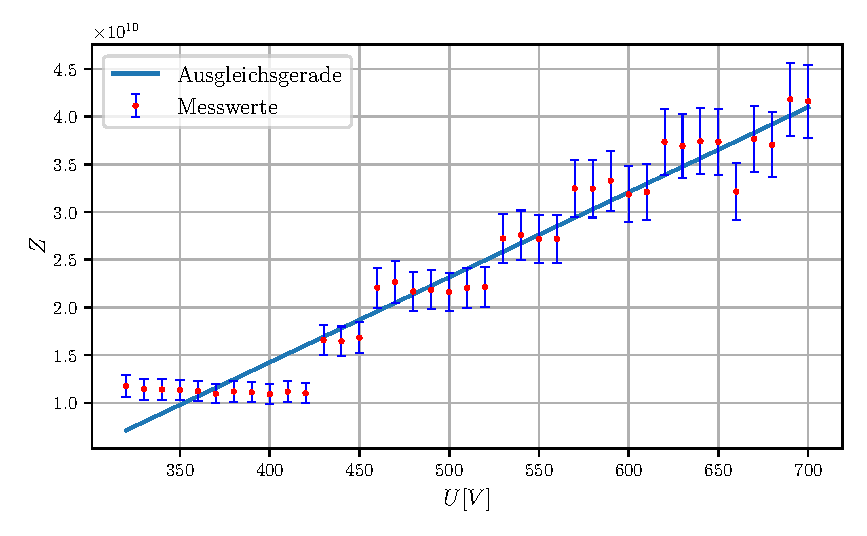
\includegraphics[width=\textwidth]{build/plot2.pdf}
  \caption{Um den Untergrund bereinigte Messwerte des Depolarisationsstroms.}
  \label{fig:plot2}
\end{figure}


